
\section{DESIGN}

In this section, we firstly introduce the basic LPSBL method.
After the basic LPSBL method is proposed, we describe the robust LPSBL method in the next subsection.
Finally, the computational complexity analysis of LPSBL is given.

\subsection{Basic LPSBL}

In this section, we introduce the basic sequence-based localization technique based on linear programming method.

Considering a sensor network in the 2D space with $N$ nodes, all nodes is $\bm{X} = \{ \bm{nod{e_1}}, \cdots ,\bm{nod{e_i}}, \cdots ,\bm{nod{e_N}}\}$, 
where any node $\bm{nod{e_i}}$ has its location coordinates denoted as $[{x_i},{y_i}]$. 
As showed in Fig. 2, an acoustic event occurs at $\bm{X_s}{\rm{ = [}}{x_s};{y_s}]$, ${d_i}$ is the distance from $nod{e_i}$ to the acoustic source $\bm{X_s}$.
The node sequence is determined by the distances from nodes to the acoustic source $\bm{X_s}$.
Given the following node sequence $NodeSeq( \cdots ,i,j, \cdots )$, ${d_i}<{d_j}$ can be inferred. We have the following inequality:
 \begin{equation} \label{equation_1}
(x_i-x_s)^2+(y_i-y_s)^2 < (x_j-x_s)^2+(y_j-y_s)^2
 \end{equation}
Then, we get
\begin{equation} \label{equation_2}
2(x_j-x_i)x_s+2(y_j-y_i)y_s<x_j^2-x_i^2+y_j^2-y_i^2
\end{equation}



Given the node sequences with $N$ node, we can get $N(N - 1)/2$ linear constraints. The
locations of nodes can be computed by solving the following linear feasibility problem:
\begin{equation}
\bm {{A}{X_s}}< \bm{{b}}
\end{equation}
where
\[\bm{A} = 
\left[
\begin{array}{lcr}
2x_2-2x_1 & 2y_2-2y_1 \\
2x_3-2x_2 & 2y_3-2y_2 \\
\quad  \quad      \vdots  &   \vdots  \\
2x_n-2x_{n-1} & 2y_n-2y_{n-1}
\end{array}
\right]
\]

\[\bm {b}=
\left[
\begin{array}{lcr}
x_2^2-x_1^2+y_2^2-y_1^2 \\
x_3^2-x_2^2+y_3^2-y_2^2 \\
  \quad \quad \quad  \vdots \\
x_n^2-x_{n-1}^2+y_n^2-y_{n-1}^2
\end{array}
\right]
\]


The problem of finding a feasible solution to a system of linear inequalities is a linear programming
problem in which the objective function is zero. 
We can find a solution to this feasibility program only if there is an embedding satisfying all of the constraints. 
We utilize the nodes sequences to set the inequality constraint.
The bound constraint in the linear programming problem is set based on the size of the network deployment area.

Describing the problem of sensor node localization in the standard form of linear programming as

 \begin{equation} \label{6}
 \quad \quad \bm {\hat X_s} = \min {\bm{c^T}\bm{X_s}}
  \end{equation}
\begin{align*}
 s.t. \   \bm {{A}{X_s}} &\le \bm {b} \\
\end{align*}
where $\bm {c}$ is zero vector.

To summarize, the LPSBL is presented in Algorithm 1. 
The input is the node sequences and anchor locations; the output is the locations of target nodes. 
Step 1 sets the objective function of the optimization problem. 
Step 2 uses the node sequence to get the inequality constraint. 
Step 3 solves the LP problem to achieve the location of target nodes.
\begin{algorithm}
\caption{LPSBL Method}
\KwIn { The location of $N$ smartphones \\
\hspace{0.41in} The node sequence of the acoustic source for\\
\hspace{0.41in} $N$ reference nodes
}
\KwOut {Location of the acoustic source}

\textbf{Step 1:} Setting objective function: setting $\bf{c} \leftarrow \bf{0}$;

\textbf{Step 2:} Constructing inequality constraint: \\ 
\hspace{0.41in} setting $\bm{A}$ and $\bm{b}$ by processing node sequence;\\
\For{$i \leftarrow 1$ \textbf{to} $N-1$}
{
\For{$j \leftarrow i+1$ \textbf{to} $N$}
{
According to inequality (\ref{equation_2}) to get inequality constraint;
}
}

\textbf{Step 3:} Solve LP problem to get the target's location.

\end{algorithm}


\subsection{LPSBL with Flip Tolerance }

    \begin{figure}[!htb]
    \centering
 \setlength{\abovecaptionskip}{-15pt}
                     \vspace{-5mm}  
 %\setlength{\belowcaptionskip}{-5pt}
    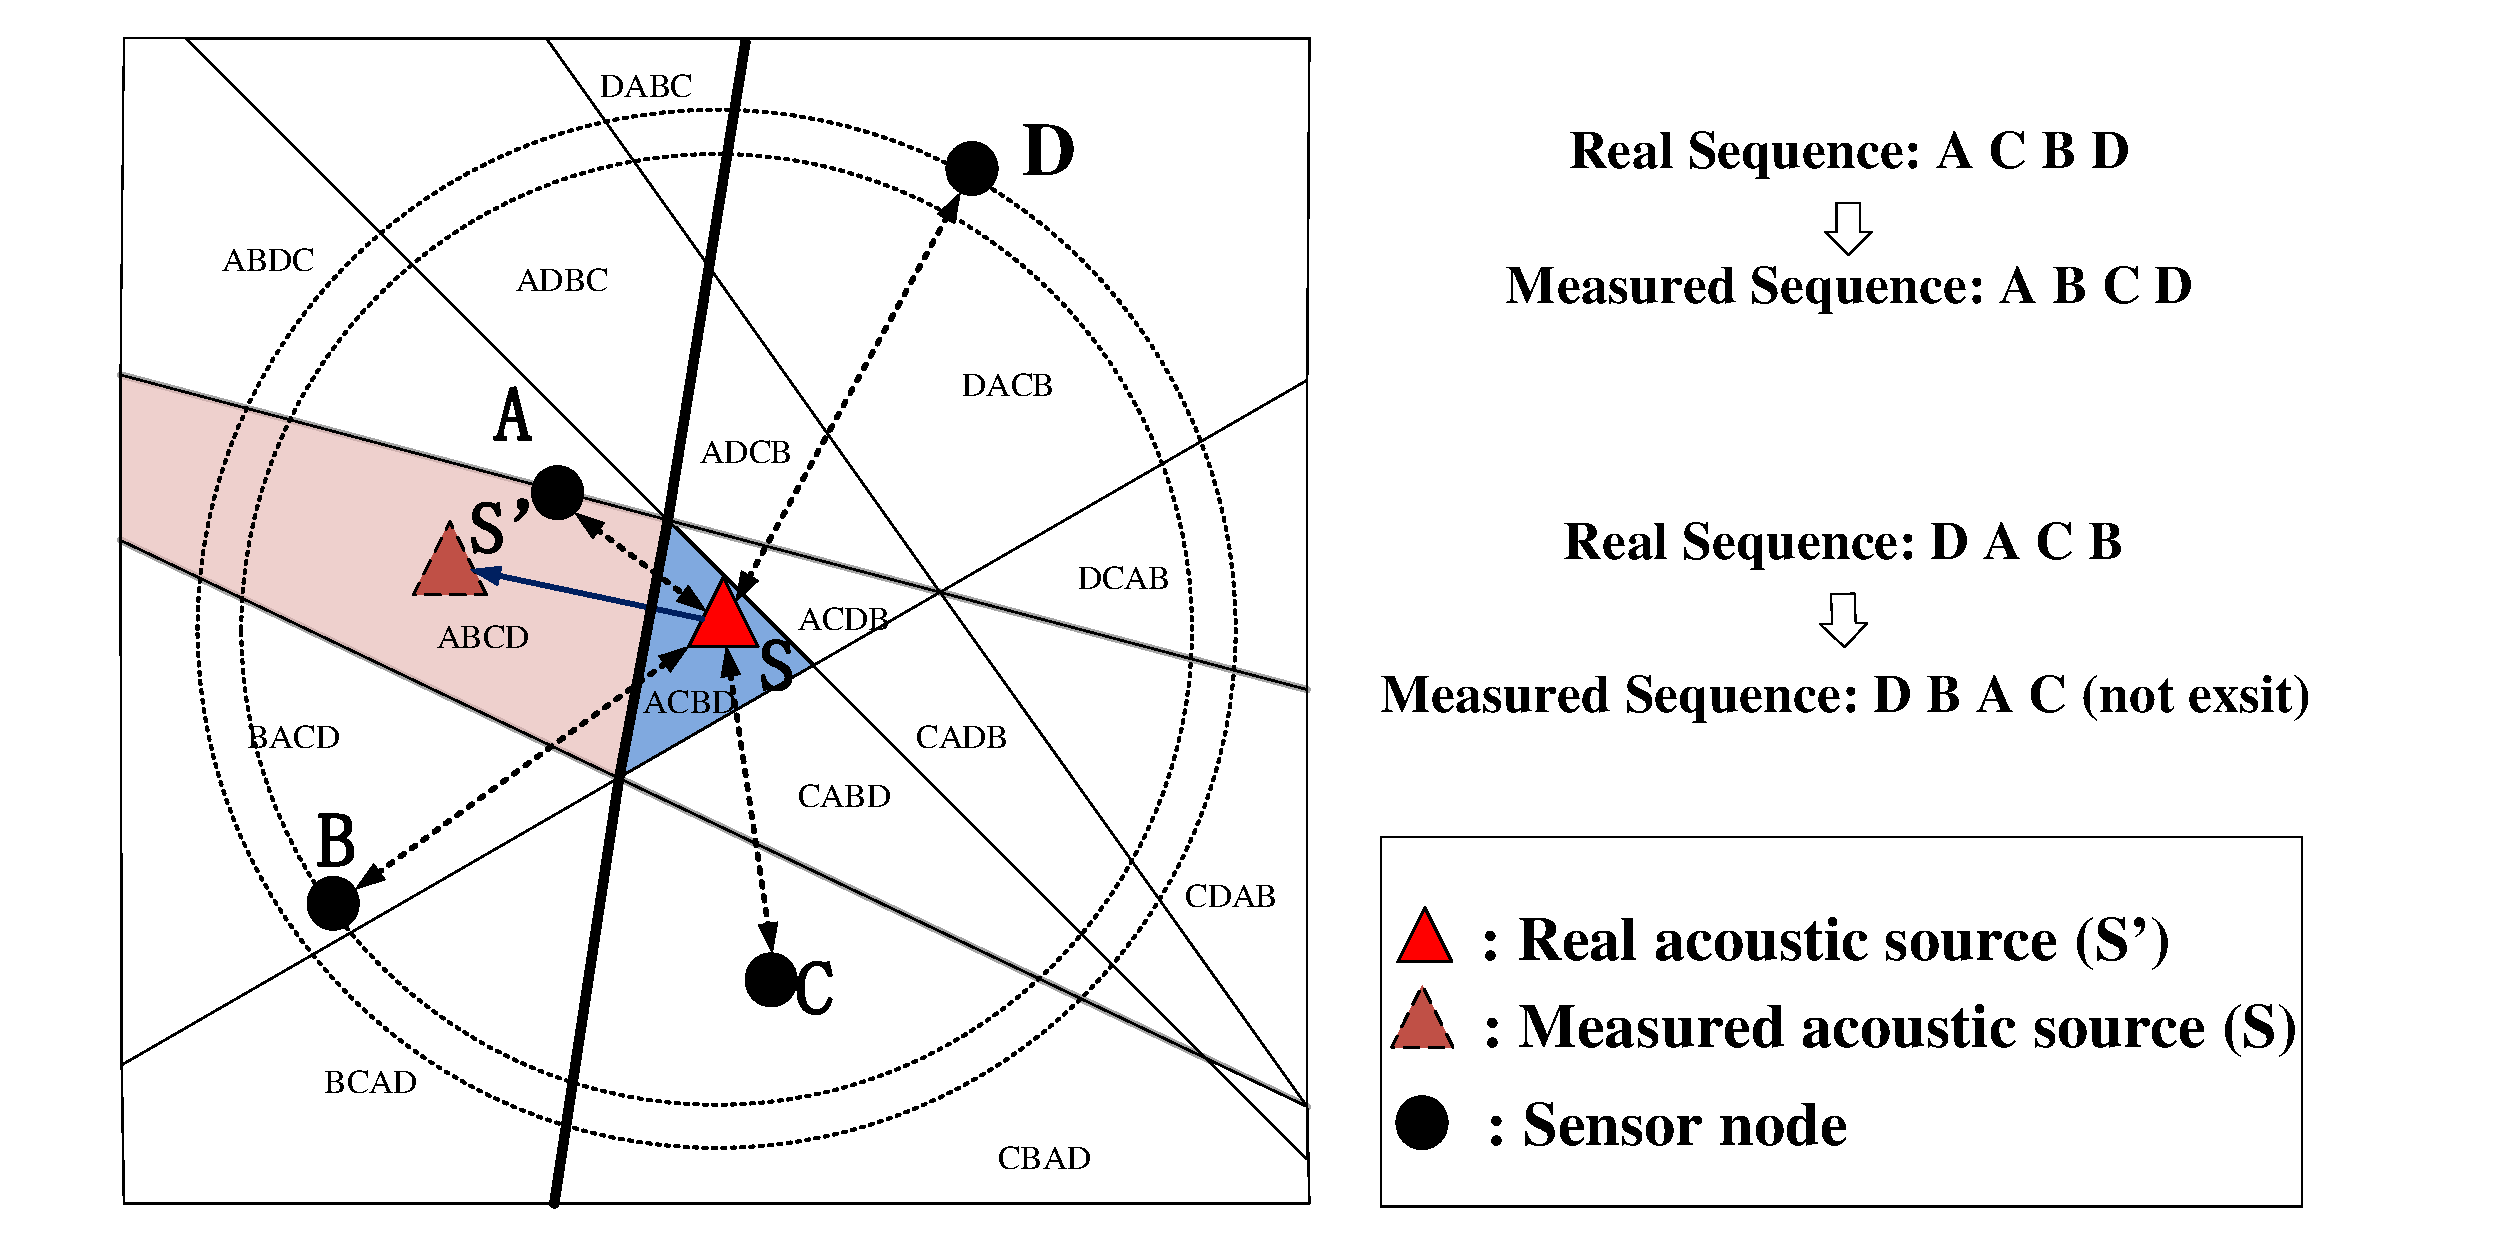
\includegraphics[height=4.5cm]{image/flip.eps} 
	\vspace{10mm}
    \caption{Flip Tolerance}
	\label{fig2}
    \vspace{-5mm}
    \end{figure}

For the sake of presentation, until now we have described LPSBL in an ideal case where a complete and perfect node sequence can be obtained. 
In this section, we describe how to make LPSBL work well under more realistic conditions. 

In the practical application, if two nodes are located too close to each other along the direction of event propagation, they detect the event almost simultaneously. 
In this case, the node ordering in the sequence may occur flip. 
For instance, the true sequence is $NodeSeq ( \cdots ,i,j, \cdots )$, but the detected sequence is $NodeSeq ( \cdots ,j,i, \cdots )$.
Algorithm 1 can find a solution to this feasibility program only if there is an embedding satisfying all of the constraints. 
However, it is impossible to find a feasible solution that satisfies all of the constraints when sequence flip occurs. 
For example, as showed in Fig. 2, the right middle region identifies by the node sequence $NodeSeq (D C A B)$. 
Once the order of node A and B occur flip in $NodeSeq (D C A B)$, the region corresponding to $NodeSeq (D C B A)$ does not exist, Algorithm 1 can not give the accurate estimation.
In this section, we propose the solution to address the problem of sequence flip using traditional convex relaxation techniques.


We thus introduce a slack variable ${\xi _{ij}}$ for each inequality constraint to allow for inequality violations.
Rewrite the inequality constraint (\ref{equation_2}) as
 \begin{equation} \label{10}
 d_i - d_j  \le  0 ; \  i,j \in S
 \end{equation}
 Relax the inequality constraint (\ref{10}) to
 \begin{equation} \label{11}
 d_i - d_j  \le  \xi _{ij} ; \  i,j \in S
 \end{equation}
 where
 \begin{math}
 \xi _{ij}  > 0
 \end{math}.
 
As a result, LPSBL with error tolerance can be formulated as a convex optimization problem with linear inequalities constraints as follows:
 \begin{equation} \label{5}
\quad \quad \quad \mathop {\min }\limits_{{x_i},{y_i}} \sum\limits_{(i,j) \in X} {{\xi _{ij}}};\  \xi _{ij} \ge 0\\
  \end{equation}
  \begin{align*}
 s.t.\   d_i - d_j  \le  \xi _{ij} \
\end{align*}
where the objective function of optimization problem is the total amount of all slacks. 

In the optimization problem expressed by the equation \eqref{5}, the problem of inequality violations can be solved by introducing a slack variable for each inequality \cite{Boyd2004}.
Therefore, the proposed LPSBL can provide the robust estimation when the problem of sequence flip occurs.








\subsection{Incremental LPSBL }

The data transmitted from the sensor node reach the the server in sequence in WSN.
The basic idea of the proposed incremental LPSBL is to ultilize the available constraints to solve the linear program.
Once the new data come, the proposed incremental LPSBL add the new constraints to refresh the location of the acoustic source by solving a
new linear program.
\begin{algorithm}
\caption{Incremental LPSBL Method}
 \KwIn { the first two data package $pack_i$ $pack_j$ \\
 \hspace{0.41in} newest data package $pack_k$ \\
 }
 \KwOut {Location of the acoustic source}
 
 \textbf{Step 1:}  Initial LP problem using the first two data package $pack_i$ $pack_j$ \\
          while (the newest data package $pack_k$ reach)\\		 
		   $pack_k$ ($ID_k$,$Location_k$,$TOA_k$)\\
\textbf{Step 2:}  Constructing inequality constraint according to the TOA of the newest data package : \\ 

\textbf{Step 3:} Solve LP problem to get the target's location.\\
       
 
 \end{algorithm}


 
 \subsection{Robust LPSBL}
 
Given the $NodeSeq (A C B D)$, the constraint is tight for AC, CB and BD, can contribute more to the localization accuracy. 
 However, compared with the constraint of AD, the the constraint of AC is subject to flip.
   % Given the following node sequence $NodeSeq( \cdots ,i,j, \cdots )$, the uncertainty of ${d_i} < {d_j}$ can be described as : 
  % \begin{equation}
  % p({d_i} < {d_j})>\alpha
  % \end{equation}
 We add the constraint of AD firstly, then process the constraints of AB and CD,  finally, the constraints of AC, CB and BD is added.
 After add the new constraint, once the optimal solution is not given, we just discard the constraint and keep the optimum before.


 
\begin{algorithm}
\caption{Robust LPSBL}
 \KwIn { the first two data package $pack_i$ $pack_j$ \\
 \hspace{0.41in} newest data package $pack_k$ \\
 }
 \KwOut {Location of the acoustic source}
 
 \textbf{Step 1:}  Initial LP problem using the first two data package $pack_i$ $pack_j$ \\
          while (the newest data package $pack_k$ reach)\\		 
		   $pack_k$ ($ID_k$,$Location_k$,$TOA_k$)\\
\textbf{Step 2:}  Constructing inequality constraint according to the TOA of the newest data package : \\ 

\textbf{Step 3:} Solve LP problem to get the target's location.\\
       
 
 \end{algorithm}
 
\subsection{Complexity Analysis}
This section provides the complexity analysis for the proposed
LPSBL design. It needs to be emphasized that
LPSBL itself adopts an asymmetric design in which sensor
nodes need only to detect and report the events. Therefore,
we only analyze the computational cost on the node sequence
processing side, where resources are plentiful.

SBL: Calculating the Kendall’s Tau
between two sequences is $O(N^2)$ operations. Since the location sequence table is of size
$O(N^4)$, searching through it takes $O(N^6)$ operations~\cite{yedavalli2008sequence}.

LPSBL: The complexity of low dimensional linear programming
with L constraints is $O(L)$\cite{Griva2009}. The number of linear constraints is $N(N-1)/2$ in LPSBL,
where $N$ is the number of nodes. Thus, the overall computation
complexity of LPSBL can be written as $O(N^2)$.



